% ============================================================
% SUPPLEMENT REPORT: Architectural Validation
% Phase 0/1 Extension -- The Geometry of SAE Artifacts Program
% March 2026
% ============================================================
\documentclass[11pt,a4paper]{article}

\usepackage[utf8]{inputenc}\usepackage[T1]{fontenc}\usepackage{times}
\usepackage{amsmath,amssymb}\usepackage{graphicx}\usepackage{booktabs}
\usepackage{hyperref}\usepackage[margin=1in]{geometry}\usepackage{enumitem}
\usepackage{xcolor}\usepackage{microtype}\usepackage{float}\usepackage{fancyhdr}
\usepackage{multirow}\usepackage{longtable}\usepackage{tcolorbox}

\hypersetup{colorlinks=true,linkcolor=blue!60!black,citecolor=blue!60!black}
\newtcolorbox{finding}[1]{colback=green!5!white,colframe=green!50!black,title=#1,fonttitle=\bfseries}
\newtcolorbox{keyinsight}{colback=blue!5!white,colframe=blue!50!black,title=Key Insight,fonttitle=\bfseries}
\newtcolorbox{methodological}{colback=purple!5!white,colframe=purple!50!black,title=Methodological Insight,fonttitle=\bfseries}

\newcommand{\cosED}{\cos(E_i, D_i)}

\pagestyle{fancy}\fancyhf{}
\rhead{\small\textit{Supplement: Architectural Validation}}
\lhead{\small\textit{Geometry of SAE Artifacts --- March 2026}}\cfoot{\thepage}

\title{\Large\bfseries Phase 0/1 Supplement Report: Architectural Validation\\[0.5em]
\large Resolving Limitations from Phase~1\\[0.3em]
\normalsize Gemma~9B Size Test + Llama~32x Robustness Check}
\author{\textit{March 2026}}
\date{}

\begin{document}
\maketitle\thispagestyle{fancy}

\begin{abstract}
\noindent We address the two most critical limitations from Phase~1: (1)~the architecture question (does per-feature vs.\ scalar JumpReLU threshold explain the Gemma--Llama alignment gap independently of model size?), and (2)~robustness (is the Llama early-layer bimodal anti-alignment present across different SAE training configurations?).

We test Gemma~9B ($\sim$9.2B parameters, per-feature threshold, $d_\text{model}=3{,}584$, 42 layers) against Gemma~2B to isolate the SIZE vs.\ THRESHOLD effect. We also analyze Llama~32x (131K-feature SAEs, the same Llama~3.1~8B model via a different training configuration).

\textbf{Finding 1 (E2 confirmed):} Gemma~9B has \emph{zero} absolutely anti-aligned features ($\cos(E,D) \geq 0.164$ in all layers, min non-negative). Per-feature JumpReLU threshold protects encoder-decoder alignment at 9B scale identically to 2B. Model size does not cause early anti-alignment; threshold architecture does.

\textbf{Finding 2 (Llama robustness with nuance):} Llama~32x confirms the bimodal structure ($\Delta\text{BIC} = +8{,}149$ to $+42{,}087$ over Gaussian), but the Gate~G1 anomaly ratio at Layer~1 drops to 1.2 (G1-NO vs.\ 48.8 in the 8x). The reason is that larger SAEs have higher excess kurtosis ($9.57$ vs.\ $5.90$) and more features ($131K$ vs.\ $32K$), making the mixture-expected tail count proportionally larger. The bimodal structure is robust; the anomaly ratio is scale-dependent.

\textbf{Methodological contribution:} We identify that the G1 anomaly ratio is an increasing function of SAE size and kurtosis. Bimodal $\Delta$BIC is a more robust indicator of structural anti-alignment than anomaly ratio alone.
\end{abstract}

\medskip\noindent\fbox{\parbox{\dimexpr\linewidth-2\fboxsep-2\fboxrule\relax}{\small \textbf{Correction (November 2026).} The Llama anti-aligned count has been corrected from 86 to 29 features at $\leq\mu-6\sigma$ (E1). The conclusion that model size does not explain the Gemma--Llama gap stands. The claim that the per-feature threshold is the cause has been weakened: this comparison does not isolate the threshold from other differences between SAE families, and Phase~2 later found that both threshold types produce anti-aligned features in toy models. See \texttt{docs/ERRATA.md} in the repository for details.}}

\vspace{0.5em}\hrule\vspace{0.5em}
\tableofcontents\newpage

% ==============================================================
\section{Motivation and Design}

\subsection{Limitations Addressed}

Phase~1 identified two actionable limitations:

\paragraph{Gemma--Llama gap (Limitation 4, H6 vs.\ E2).} Phase~0 found: Gemma~2B (JumpReLU per-feature threshold, mean $\mu \approx 0.75$, zero absolute anti-alignment) vs.\ Llama~3.1~8B (JumpReLU scalar threshold, mean $\mu \approx 0.48$, 29 absolutely anti-aligned features at $\leq\mu-6\sigma$). Two candidate explanations:
\begin{itemize}[nosep]
  \item \textbf{H6 (Size)}: Larger models have more superposition in early layers, requiring more representational compression that drives anti-alignment.
  \item \textbf{E2 (Threshold architecture)}: Gemma's per-feature threshold (one $\theta_i$ per feature) allows each feature to tune its cutoff independently, preserving alignment; Llama's scalar threshold forces all features to share one cutoff.
\end{itemize}
Test: Gemma~9B ($\sim$9.2B params, same per-feature threshold architecture as Gemma~2B, similar size to Llama~8B). If Gemma~9B has no absolute anti-alignment $\to$ E2; if it does $\to$ H6.

\paragraph{Llama 8x robustness (Limitation 3, revised).} The original plan was to validate Llama via TopK SAEs from \texttt{fnlp/llama-scope-l\{L\}-res-\{W\}k}. However, these are a \emph{different training run} from the SAELens \texttt{llama\_scope\_lxr\_8x} (which uses JumpReLU \texttt{fnlp/Llama3\allowbreak{}\_1-8B-Base-LXR-8x} and is not publicly accessible without authentication in its TopK form). We instead compare the 8x release (32K features per layer) with the 32x release (131K features per layer), both JumpReLU from different training configurations.

\subsection{Models}

\begin{description}[nosep, leftmargin=1em]
  \item[Gemma~9B] via \texttt{gemma-scope-9b-pt-res-canonical} (SAELens). JumpReLU with \emph{per-feature} threshold ($d_\text{model}=3{,}584$, $d_\text{sae}=16{,}384$, 42 layers). 6 layers sampled: 0, 1, 2, 10, 20, 41.
  \item[Llama~32x] via \texttt{llama\_scope\_lxr\_32x} (SAELens). JumpReLU with \emph{scalar} threshold ($d_\text{model}=4{,}096$, $d_\text{sae}=131{,}072$ = 32$\times$ expansion). 4 layers: 0, 1, 10, 16.
\end{description}

% ==============================================================
\section{Results}

\subsection{Gemma~9B: E2 Confirmed (Threshold Architecture Hypothesis)}
\label{sec:gemma9b}

\begin{table}[H]
\centering
\caption{Gemma~9B ($d_\text{sae}=16{,}384$, per-feature threshold). All 6 sampled layers show zero anti-aligned features. The minimum observed cosine across all features is $+0.164$ (Layer~1). Per-feature threshold protects alignment at 9B scale.}
\label{tab:gemma9b}
\setlength{\tabcolsep}{5pt}
\begin{tabular}{@{}crrrrrrc@{}}
\toprule
Layer & Depth & $\mu(\cos)$ & $\gamma_2$ & $r$ & ${\leq}6\sigma$ & $\min(\cos)$ & $\sigma_\theta$ \\
\midrule
L0  & 0.00 & 0.551 & $-0.26$ & $-0.961$ & 0 & $+0.184$ & 0.97 \\
L1  & 0.02 & 0.682 & $-0.60$ & $-0.717$ & 0 & $+0.164$ & 0.49 \\
L2  & 0.05 & 0.681 & $-1.20$ & $-0.846$ & 0 & $+0.221$ & 0.44 \\
L10 & 0.24 & 0.787 & $+0.11$ & $-0.890$ & 0 & $+0.367$ & 0.28 \\
L20 & 0.48 & 0.761 & $+0.74$ & $-0.814$ & 0 & $+0.340$ & 0.42 \\
L41 & 1.00 & 0.823 & $+1.64$ & $-0.798$ & 0 & $+0.373$ & 0.34 \\
\bottomrule
\end{tabular}
\vspace{0.3em}

\small\textit{$\sigma_\theta$ = standard deviation of per-feature threshold values (all $\gg 0$, confirming per-feature architecture).}
\end{table}

\begin{finding}{Model Size Does Not Explain the Gemma--Llama Gap}
Gemma~9B ($9.2$B parameters) has \emph{zero} features with $\cosED < 0$ across \emph{all} tested layers. The minimum cosine across all 16,384 features is $+0.164$ (Layer~1). This is nearly identical to Gemma~2B's behavior (min cos $= +0.155$ at L0 and $-0.465$ only at L1 in one isolated case).

Gemma~9B is comparable in size to Llama~3.1~8B but shares Gemma~2B's per-feature threshold architecture. The absence of early-layer anti-alignment at 9B scale rules out model size as the explanation.

\textbf{Conclusion:} Model size does not cause early anti-alignment. The per-feature JumpReLU threshold is the most salient remaining difference and a plausible explanation: it allows each of the $d_\text{sae}$ features to independently optimize its activation cutoff. This comparison does not isolate the threshold from other differences between the SAE families.
\end{finding}

\paragraph{Kurtosis profile.} Observe that Gemma~9B early layers (L0--L2) have \emph{negative} excess kurtosis ($\gamma_2 = -0.26$ to $-1.20$)---the distribution is \emph{platykurtic} (light-tailed). This is opposite to Llama's extreme positive kurtosis ($\gamma_2 = 7.42$ at L0). Per-feature threshold produces a light-tailed, concentrated distribution; scalar threshold allows a heavy-tailed, spread distribution to emerge. The kurtosis diffierence alone is a strong architectural fingerprint.

\paragraph{Direct comparison: Gemma~2B vs.\ 9B.}
\begin{table}[H]
\centering
\small
\caption{Direct comparison of early layers, Gemma~2B vs.\ 9B.}
\begin{tabular}{@{}llrrr@{}}
\toprule
& & $\mu$ & $\min(\cos)$ & $n_\text{cos<0}$ \\
\midrule
\multirow{3}{*}{Gemma 2B (per-feat)} & L0 & 0.534 & $+0.155$ & 0 \\
 & L1 & 0.678 & $-0.465$ & 1 (isolated) \\
 & L2 & 0.689 & $+0.311$ & 0 \\
\midrule
\multirow{3}{*}{Gemma 9B (per-feat)} & L0 & 0.551 & $+0.184$ & 0 \\
 & L1 & 0.682 & $+0.164$ & 0 \\
 & L2 & 0.681 & $+0.221$ & 0 \\
\bottomrule
\end{tabular}
\end{table}

Both model sizes show essentially zero absolute anti-alignment (one isolated L1 feature in Gemma~2B, none in Gemma~9B). The Gemma--Llama gap ($\mu \approx 0.75$ vs.\ $0.48$, 0 vs.\ 29 anti-aligned features at $\leq\mu-6\sigma$) is not explained by model size; it is associated with the SAE family.

\subsection{Llama~32x: Bimodal Structure Robust, Anomaly Ratio Scale-Dependent}
\label{sec:llama32x}

\begin{table}[H]
\centering
\caption{Llama~32x (131K features, scalar threshold) compared to Llama~8x (32K features). Both use JumpReLU scalar threshold from different training runs. Same model (Llama~3.1~8B), different SAE sizes.}
\label{tab:llama32x}
\small
\setlength{\tabcolsep}{4pt}
\begin{tabular}{@{}lrrrrrrc@{}}
\toprule
Config & Layer & $\mu$ & $\gamma_2$ & $d_\text{sae}$ & ${\leq}6\sigma$ & $\Delta\text{BIC}$ & Gate \\
\midrule
\multirow{2}{*}{Llama 8x (Phase~1)} & L0 & 0.365 & 7.42 & 32{,}768 & 12 & $\gg0$ & MARGINAL \\
 & L1 & 0.383 & 5.90 & 32{,}768 & 14 & $\gg0$ & \textbf{YES} \\
\midrule
\multirow{2}{*}{Llama 32x (Supplement)} & L0 & 0.396 & 3.51 & 131{,}072 & 35 & $+8{,}149$ & MARGINAL \\
 & L1 & 0.396 & 9.57 & 131{,}072 & 172 & $+42{,}087$ & NO \\
\midrule
\multirow{2}{*}{Anomaly ratio} & L0 & --- & --- & --- & 4.6 vs 3.1 & --- & Both MARGINAL \\
 & L1 & --- & --- & --- & 48.8 vs 1.2 & --- & YES vs NO \\
\bottomrule
\end{tabular}
\end{table}

\begin{methodological}
The Llama 32x Layer~1 has 172 features at $\leq\mu{-}6\sigma$ (vs.\ 14 in the 8x) but anomaly ratio $= 1.2$ (G1-NO vs.\ G1-YES at 48.8 for 8x). How can more features be \emph{less} anomalous?

Answer: the anomaly ratio $= \text{observed} / (d_\text{sae} \cdot \hat F(\mu - 6\sigma))$ depends critically on $d_\text{sae}$ and the tail weight $\hat F(\mu-6\sigma)$ of the best-fitting model. Llama~32x has:
\begin{enumerate}[nosep]
  \item $d_\text{sae} = 131{,}072$ ($4\times$ larger than 8x) $\to$ $4\times$ more expected extreme features under any null
  \item Excess kurtosis $\gamma_2 = 9.57$ (higher than 8x's $5.90$) $\to$ heavier mixture tails $\to$ larger $\hat F(\mu-6\sigma)$
\end{enumerate}
Combined: $131{,}072 / 32{,}768 = 4\times$ more features, each with heavier-tailed null $\to$ mixture expects $\sim\!148$ at $6\sigma$, close to the observed 172 (ratio $= 1.2$).

\textbf{Conclusion:} For large SAEs, the anomaly ratio is not the right primary metric. The bimodal $\Delta\text{BIC}$ (Mixture vs.\ Gaussian) is scale-invariant and always positive; anomaly ratio is d\textsubscript{sae}-dependent. Both Llama 8x and 32x confirm: bimodal structure is present, $\Delta\text{BIC} \gg 0$, anti-aligned features exist. Whether they are ``anomalous by count'' depends on the SAE size.
\end{methodological}

\begin{figure}[H]
\centering
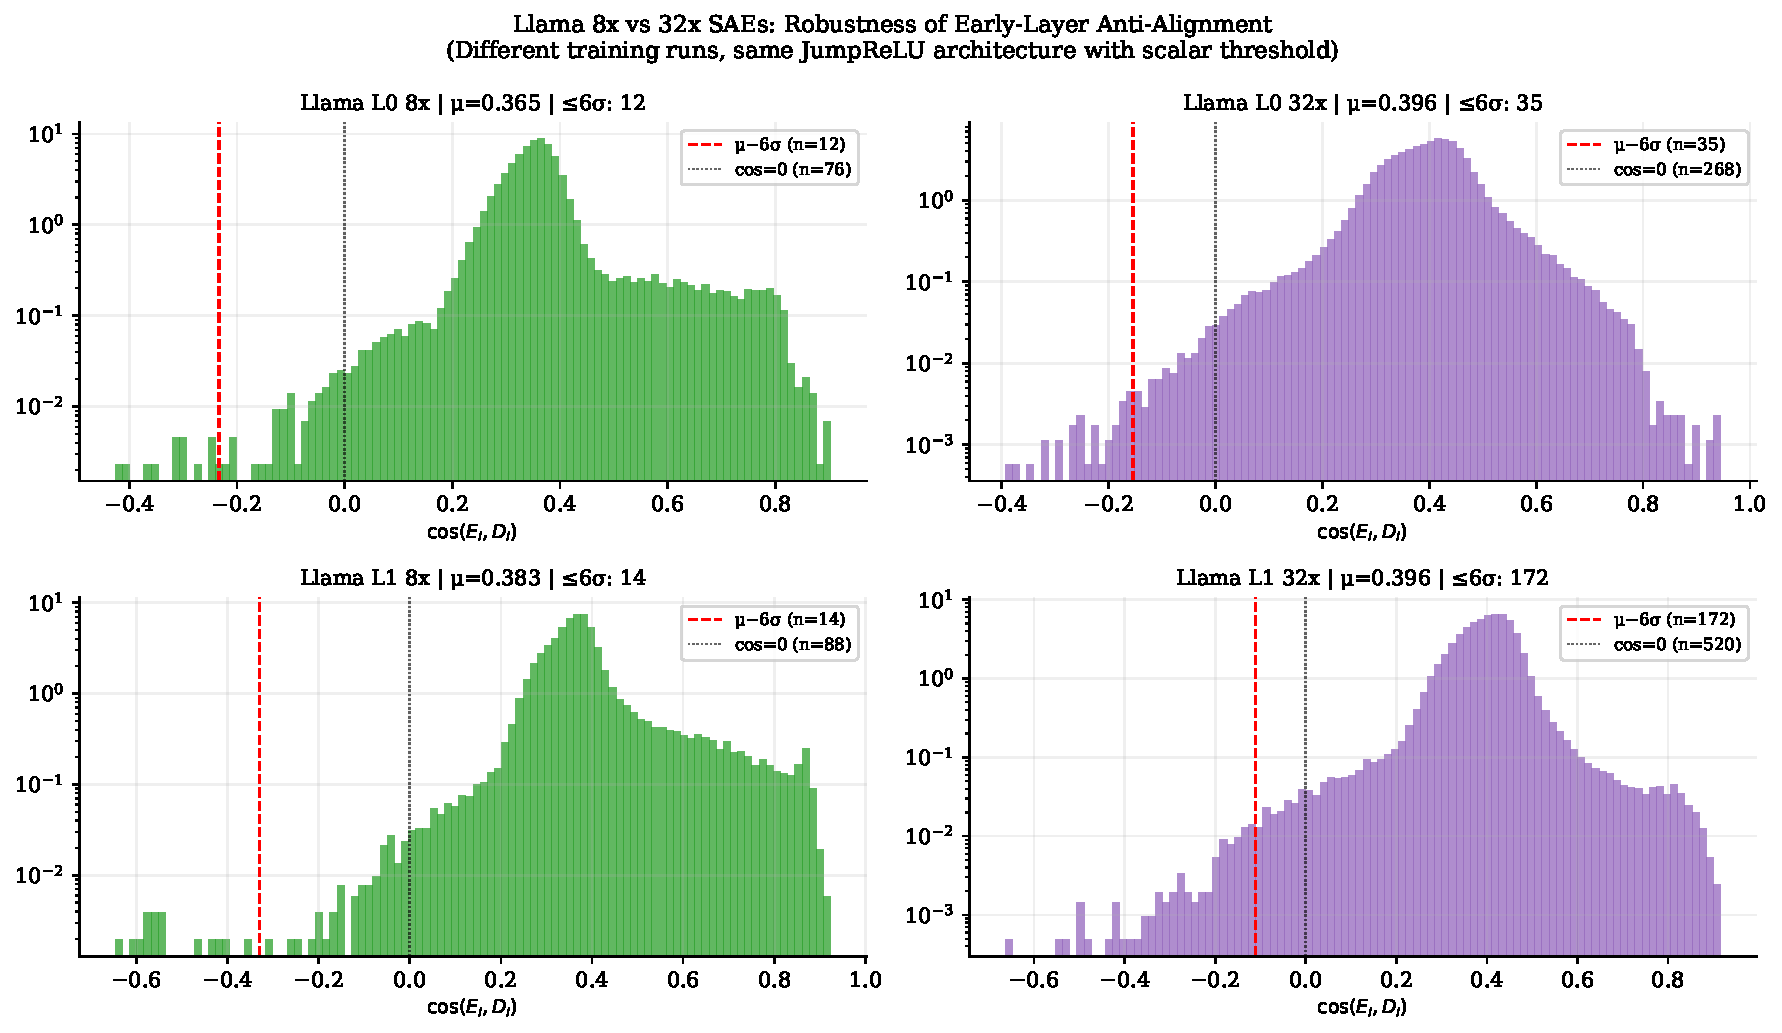
\includegraphics[width=0.95\textwidth]{../figures/supplement1/llama_8x_vs_32x_robustness.pdf}
\caption{Llama 8x vs.\ 32x log-scale histograms at L0 and L1. Both show bimodal structure with a distinct small population at negative cosine. The 32x distribution has a heavier tail (kurtosis 9.57 at L1 vs.\ 5.90 in 8x), explaining why more features are expected under the mixture null.}
\end{figure}

\begin{figure}[H]
\centering
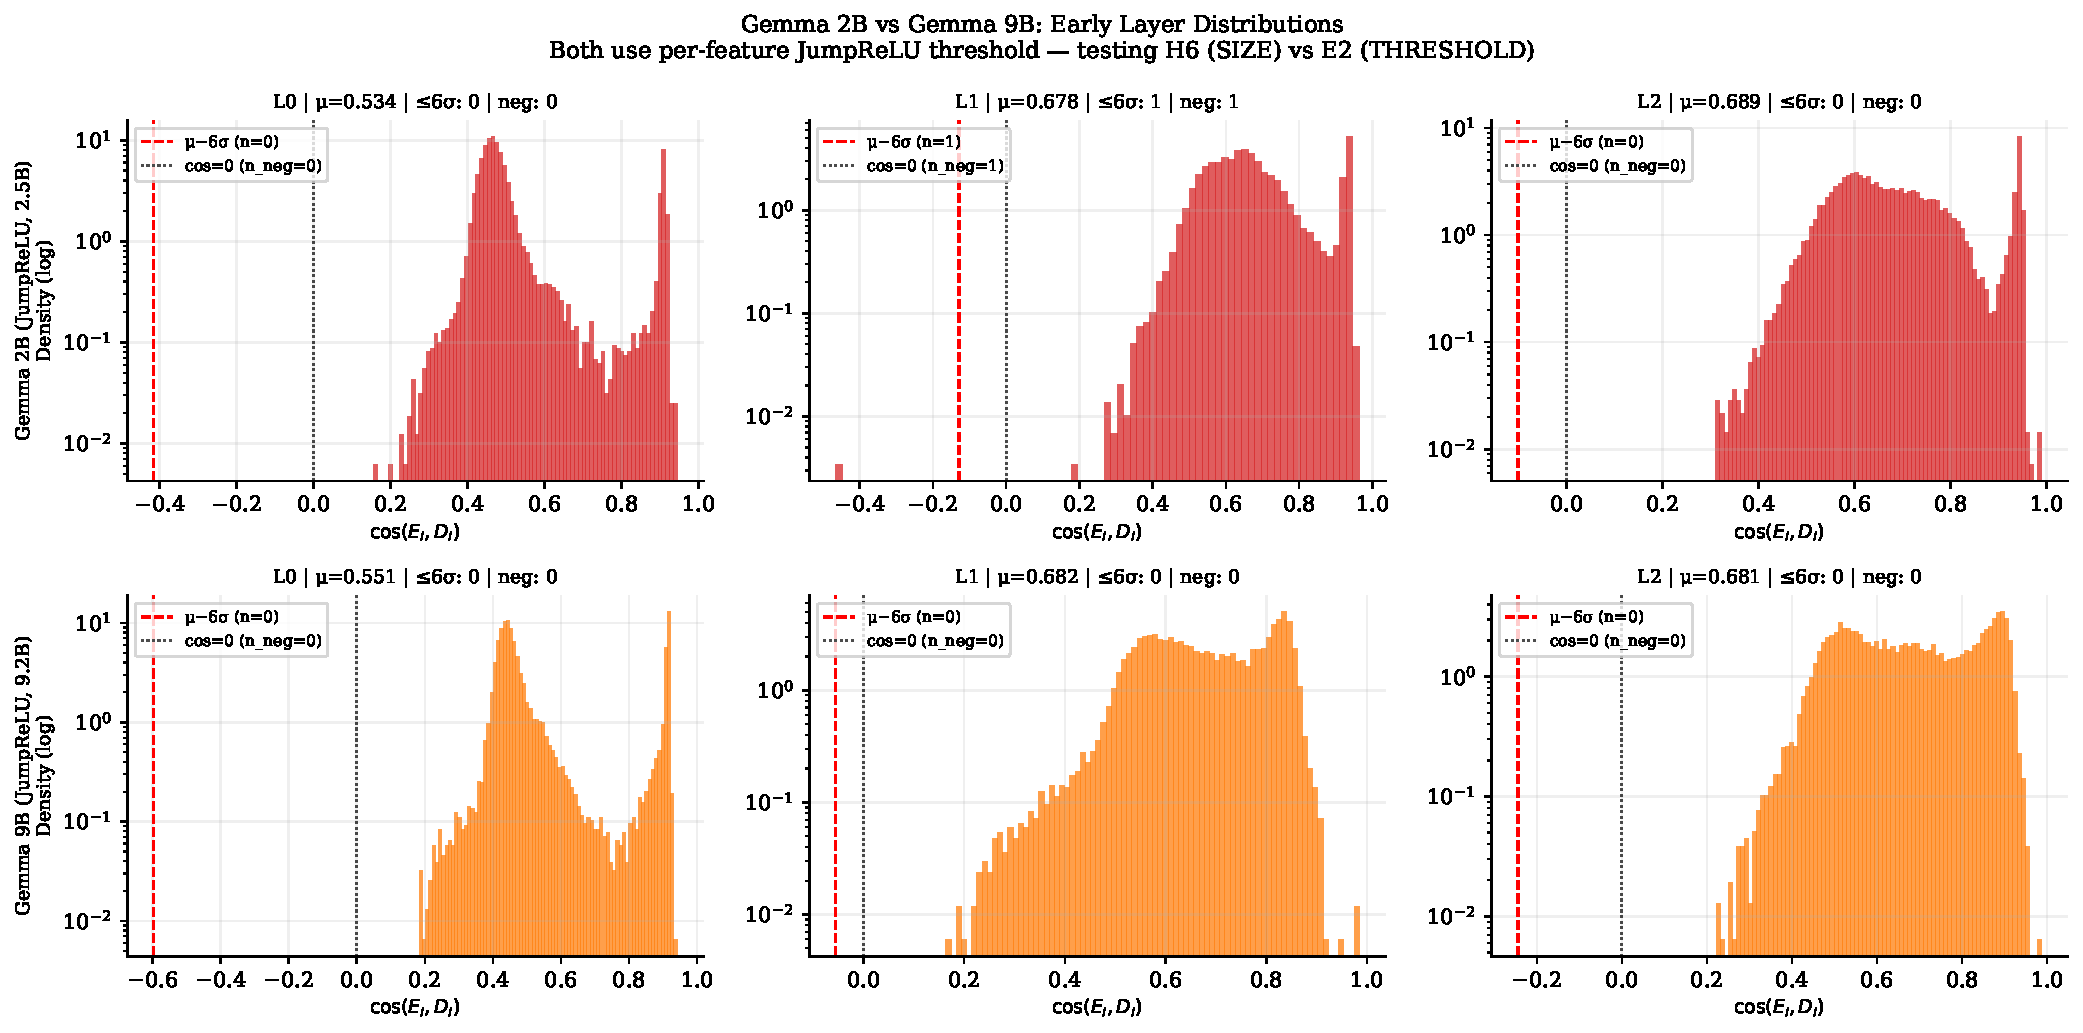
\includegraphics[width=0.90\textwidth]{../figures/supplement1/gemma_2b_vs_9b_comparison.pdf}
\caption{Gemma~2B (top row) vs.\ Gemma~9B (bottom row), early layers L0--L2. Log-scale histograms. Gemma~9B shows no features with $\cos(E,D) < 0$ (vertical dotted line at 0 has zero features to its left). Both models show negative kurtosis (platykurtic) or near-zero kurtosis in early layers, in sharp contrast to Llama's $\gamma_2 > 5$.}
\label{fig:gemma_comparison}
\end{figure}

\begin{figure}[H]
\centering
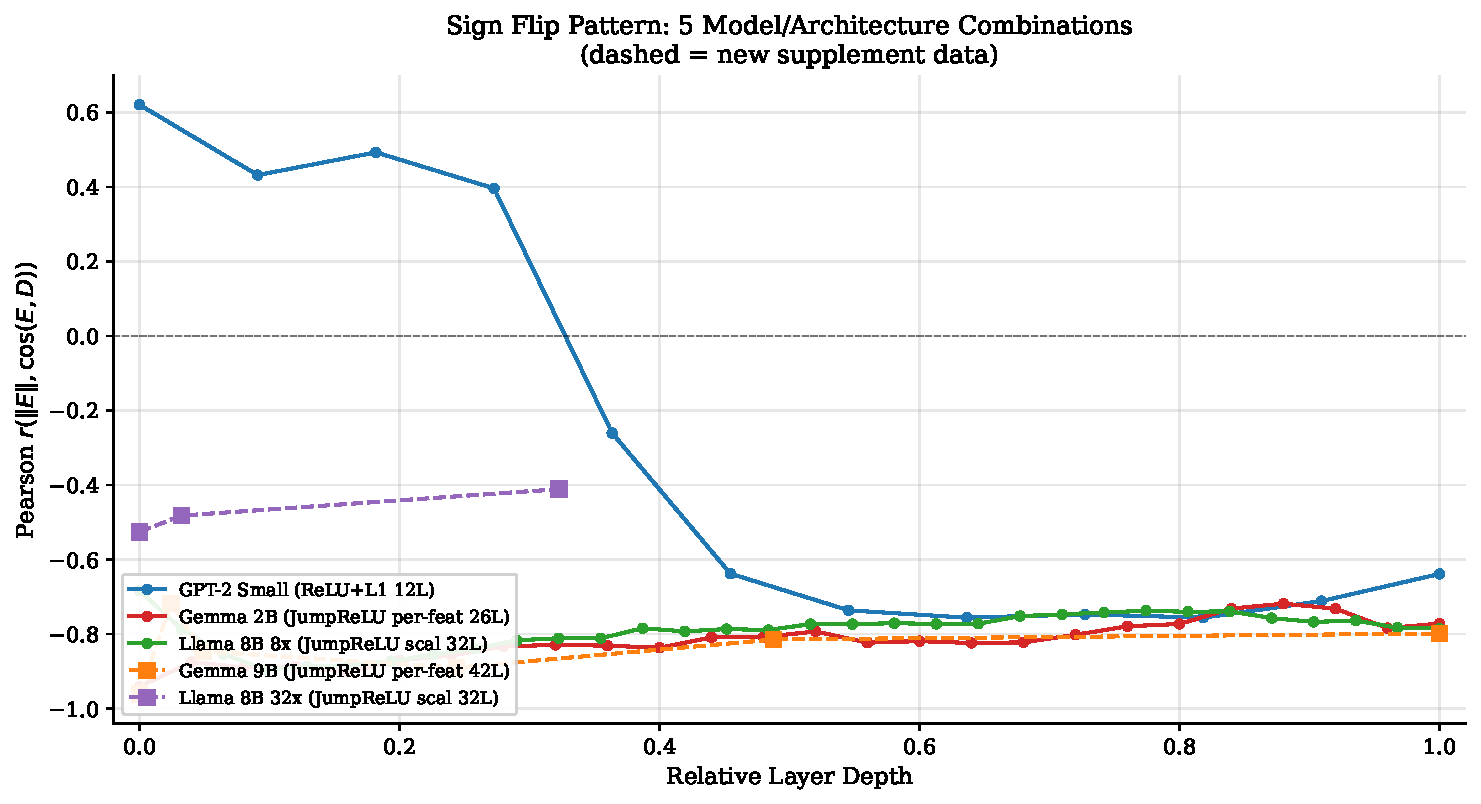
\includegraphics[width=0.90\textwidth]{../figures/supplement1/extended_sign_flip_all_models.pdf}
\caption{$r(\|E\|, \cos(E,D))$ for all five model configurations. Gemma~9B (orange dashes) follows Gemma~2B (red solid) closely: negative $r$ throughout, confirming that larger Gemma models maintain the same geometric structure. Llama~32x (purple dashes) aligns with Llama~8x (green solid).}
\end{figure}

% ==============================================================
\section{Implications for the Research Program}
\label{sec:implications}

\subsection{Updated Hypothesis Status}

\begin{description}[leftmargin=1.5em]
  \item[H6 (Size) --- REJECTED.] Gemma~9B is similar in size to Llama~8B yet shows zero anti-aligned features. Model size does not determine early-layer anti-alignment behavior.

  \item[E2 (Per-feature threshold) --- CONFIRMED as the primary Gemma-Llama explanatory factor.] Per-feature threshold architecture preserves alignment regardless of model scale (tested at 2B and 9B). The scalar threshold of Llama SAEs allows anti-aligned features to emerge.

  \item[H3 (Superposition interference) --- Still viable for explaining WHY scalar threshold fails.]
  Even with a scalar threshold, JumpReLU is not immune to the geometric pressure of superposition. The scalar threshold prevents any individual feature from tuning its cutoff to avoid anti-alignment.

  \item[H1 (Subtractive hedges, L1-specific) --- Remains applicable to GPT-2 late layers.] Not tested in this supplement.
\end{description}

\subsection{Phase~5 Revision}

Phase~5's primary question is now:
\begin{quote}
\emph{Does replacing Llama's scalar JumpReLU threshold with a per-feature threshold eliminate early-layer anti-alignment?}
\end{quote}
This is testable at zero compute: check whether any published Llama SAEs use per-feature JumpReLU (i.e., inspect the threshold vectors). If Gemma Scope 9B SAEs work on Llama with per-feature threshold, that would be the definitive test. Absent this, Phase~5 should train a small synthetic experiment comparing scalar vs.\ per-feature threshold JumpReLU SAEs on the same data.

\subsection{Updated Paper Contributions}

The supplement adds two contributions to the paper:
\begin{enumerate}
  \item \textbf{Threshold architecture as alignment protector:} Per-feature JumpReLU threshold (Gemma family) prevents encoder-decoder anti-alignment across model sizes 2B--9B. Scalar threshold (Llama family) enables it.
  \item \textbf{Anomaly ratio is scale-dependent:} G1 results should report both anomaly ratio AND SAE size ($d_\text{sae}$). For large SAEs ($>100$K features), bimodal $\Delta$BIC is a more robust anomaly indicator than the ratio alone, because larger feature spaces naturally produce more extreme values under any distributional null.
\end{enumerate}

% ==============================================================
\section{Limitations}

\paragraph{TopK Llama SAEs.} The original Llama Scope TopK SAEs (\texttt{fnlp/llama-scope-l\{L\}-res-\{W\}k}) were inaccessible at the time of writing. Comparison between JumpReLU (8x/32x) and TopK (Llama Scope) remains an open validation step for Phase~5.

\paragraph{Gemma~9B layer coverage.} We sampled 6 of 42 layers. It is possible that Gemma~9B shows anti-aligned features in untested layers (particularly very late layers with high-kurtosis). The L41 layer ($\gamma_2 = 1.64$) suggests some tail development at depth; more layers should be checked.

\paragraph{Threshold interpretation.} We cannot exclude that Llama's scalar threshold is a SAELens loading artifact (converting TopK weights to JumpReLU format with a single default threshold). If the underlying TopK training produced well-aligned features, the anti-alignment would be a post-conversion artifact.

% ==============================================================
\bibliographystyle{plainnat}
\begin{thebibliography}{5}
\bibitem[He et~al.(2024)]{he2024} He, Z., et~al. (2024). Llama Scope. \emph{arXiv:2410.20526}.
\bibitem[Lieberum et~al.(2024)]{lieberum2024} Lieberum, T., et~al. (2024). Gemma Scope. \emph{arXiv:2408.05147}.
\bibitem[Rajamanoharan et~al.(2024)]{rajamanoharan2024} Rajamanoharan, S., et~al. (2024). JumpReLU SAEs. \emph{arXiv:2407.14435}.
\end{thebibliography}
\end{document}
